\let\negmedspace\undefined
\let\negthickspace\undefined
\documentclass[journal,12pt,onecolumn]{IEEEtran}
\usepackage{cite}
\usepackage{amsmath,amssymb,amsfonts,amsthm}
\usepackage{algorithmic}
\usepackage{graphicx}
\graphicspath{{./figs/}}
\usepackage{textcomp}
\usepackage{xcolor}
\usepackage{txfonts}
\usepackage{listings}
\usepackage{enumitem}
\usepackage{mathtools}
\usepackage{gensymb}
\usepackage{comment}
\usepackage{caption}
\usepackage[breaklinks=true]{hyperref}
\usepackage{tkz-euclide} 
\usepackage{listings}
\usepackage{gvv}                                        
\usepackage[latin1]{inputenc}     
\usepackage{xparse}
\usepackage{color}                                            
\usepackage{array}                                            
\usepackage{longtable}                                       
\usepackage{calc}                                             
\usepackage{multirow}
\usepackage{multicol}
\usepackage{hhline}                                           
\usepackage{ifthen}                                           
\usepackage{lscape}
\usepackage{tabularx}
\usepackage{array}
\usepackage{float}


\begin{document}

\title{4.7.62}
\author{AI25BTECH11001 - ABHISEK MOHAPATRA}
{\let\newpage\relax\maketitle}
	 	\textbf{Question}:
Find the equation of the plane which passes through the point (5,2,-4) and perpendicular the line with direction ratios 2,3,-1.


		\textbf{Solution:} let the equation of the plane be 
\begin{align}
		\vec{n}^\top\vec{x} = c
\end{align}

as per the question, $\vec{n} = \myvec{2\\3\\-1}$ and a point ,let $\vec{P} = \myvec{5\\2\\-4}$ 

so putting the values in the equation,
\begin{align}
		\myvec{2\\3\\-1}^\top\myvec{5\\2\\-4} = c\\
		\Rightarrow c = 10 + 6 +4 = 20
\end{align}
so the required equation is
\begin{align}
		\myvec{2&3&-1}\vec{x} = 20
\end{align}

Graph:
\begin{figure}[h!]
	\centering
	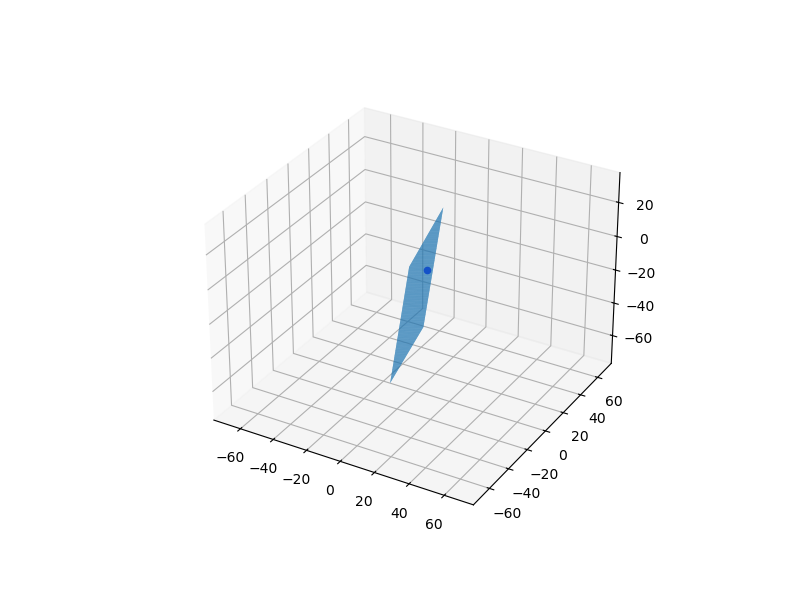
\includegraphics[width=0.7\linewidth]{img.png}
\end{figure}
\end{document}
